\documentclass[tikz, border=10pt]{standalone}

\usepackage{tikz}
\usepackage{xcolor}
\usepackage{amsmath, amsfonts, amssymb, mathtools}
\usepackage{mathpazo}

\begin{document}
    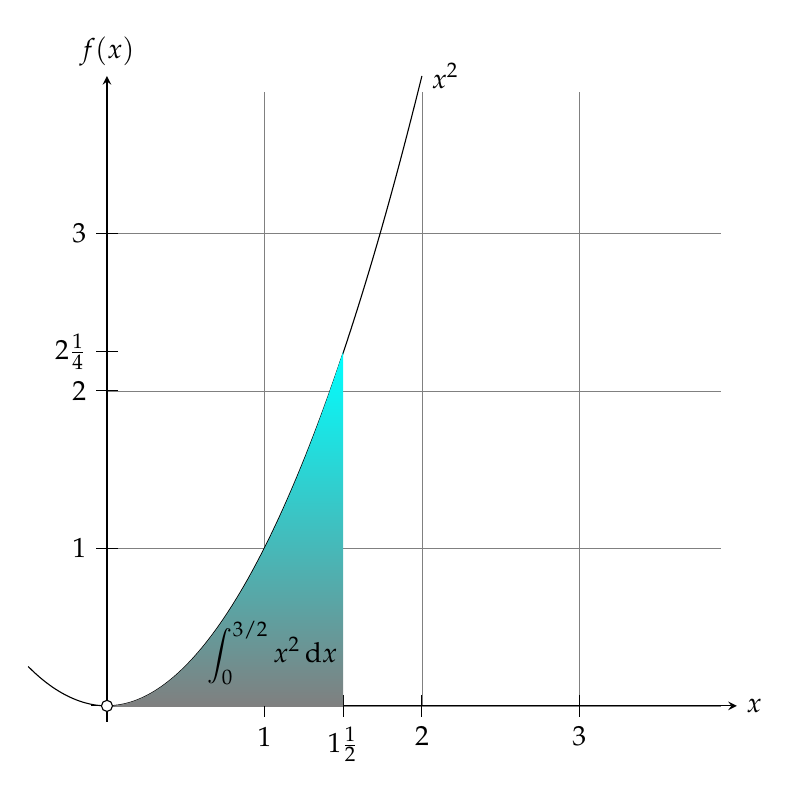
\begin{tikzpicture}[scale=2]
        \draw[style=help lines] (0, 0) grid (3.9, 3.9);
        \draw[->, >=stealth] (-0.1, 0) -- (4, 0) node[right] {$x$};
        \draw[->, >=stealth] (0, -0.1) -- (0, 4) node[above] {$f(x)$};
        
        \foreach \x/\xtext in {1, 1.5/1\frac{1}{2}, 2, 3}
            \draw[shift={(\x, 0)}] (0, 2pt) -- (0, -2pt) node[below] {$\xtext$};
        \foreach \y/\ytext in {1, 2, 2.25/2\frac{1}{4}, 3}
            \draw[shift={(0, \y)}] (2pt, 0) -- (-2pt, 0) node[left]{$\ytext$};
            
        \draw (-0.5, 0.25) parabola bend (0, 0) (2, 4) node[right] {$x^2$};
        \shade[top color=cyan, bottom color=gray] (0, 0) parabola (1.5, 2.25) |- (0, 0);
        \draw (1.05, 2pt) node[above]{$\displaystyle\int_0^{3/2}x^2\!\mathop{}\mathrm{d}x$};
        
        \filldraw[fill=white, draw] (0, 0) circle (1pt);
    \end{tikzpicture}
\end{document}